\chapter{Spark SR1020}
\label{cha:spark}
Spark Microsystems' central offerings are the SR1010 and SR1020 transceivers. These are integrated short-range UWB devices recognized for their low power consumption and rapid response times. They are designed for robust, energy-efficient communication in the license-free Ultra-Wideband spectrum, which spans 3.1 to 9.25 GHz. Note that the exact frequencies allowed without licensing vary by country. Spark provides documentation on their website about how the FCC regulations apply to their products. Figure 3.1 showcases European regulations. For this study, we limited our tests to frequencies between 6.5 GHz and 8.5 GHz.

\begin{figure}
\centering
    \begin{subfigure}[b]{.49\textwidth}
        \centering
        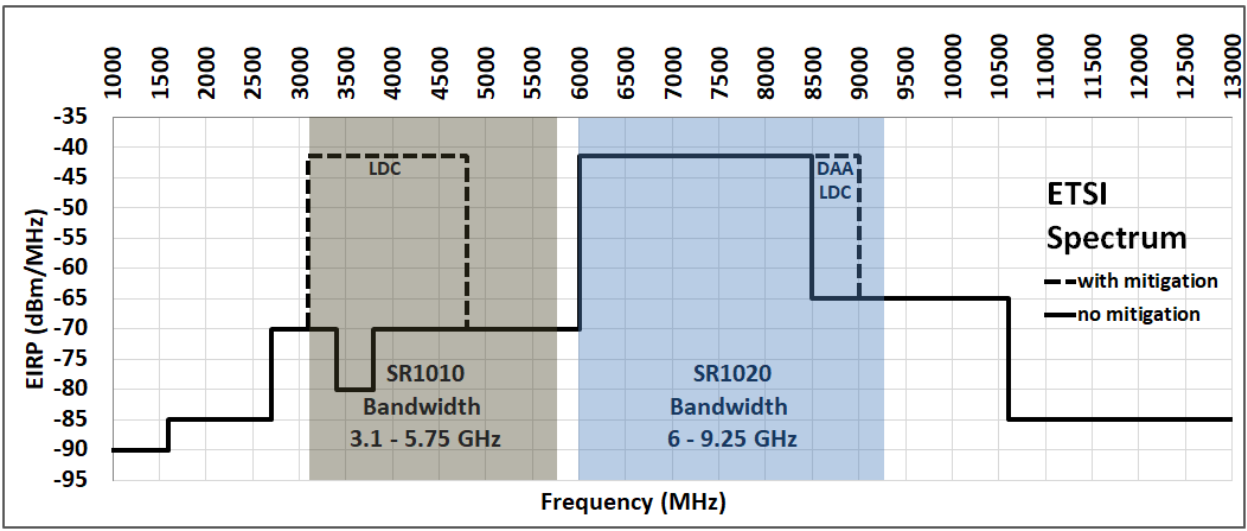
\includegraphics[width=\textwidth]{images/FCC spectrum ETSI.png}
        \caption{Maximum mean emission levels for UWB communications devices by ETSI.}
        \label{fig:spark_ETSI}
    \end{subfigure}
    \hfill
    \centering
    \begin{subfigure}[b]{.49\textwidth}
        \centering
        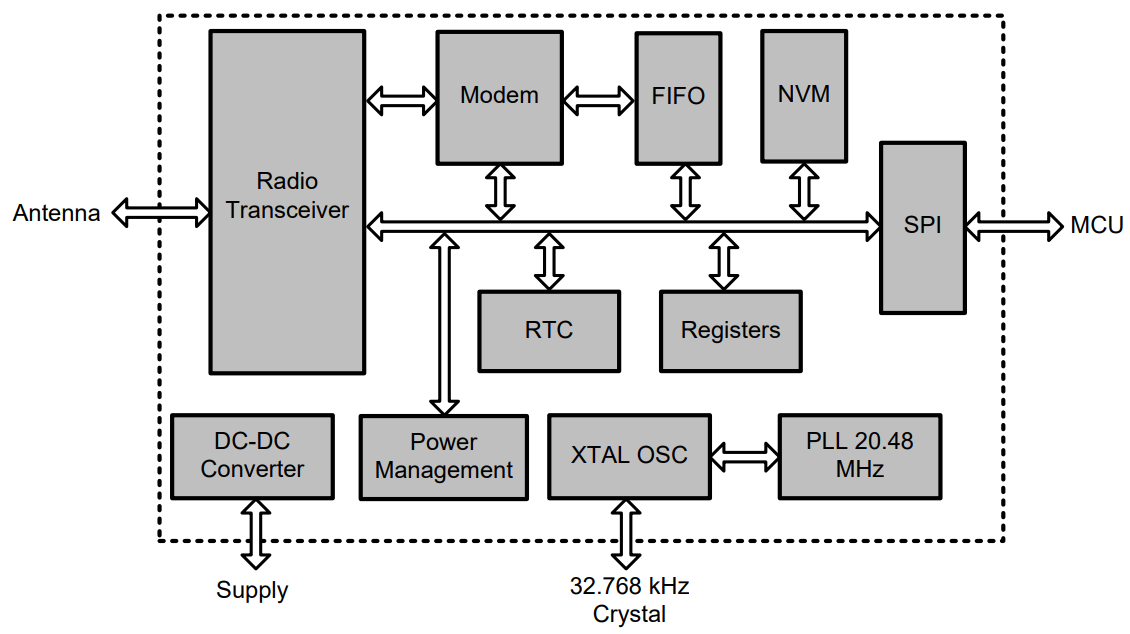
\includegraphics[width=\textwidth]{images/radio picture datasheet.png}
        \caption{System Block Diagram}
        \label{fig:system_block_diagram}
    \end{subfigure}
    \hfill
    \begin{subfigure}[b]{.7\textwidth}
        \centering
        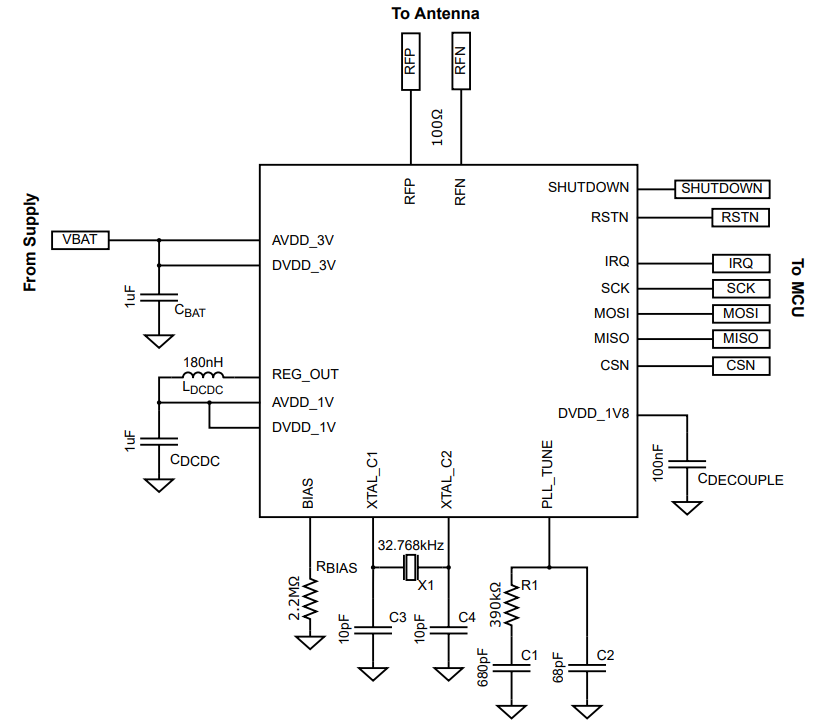
\includegraphics[width=\textwidth]{images/radio circuit datasheet.png}
        \caption{Spark SR1020 Circuit.}
        \label{fig:radio_circuit}
    \end{subfigure}
    \caption{SR1020 Radios Circuit}
    \label{fig:sr1020_radios}
\end{figure}


%2 [depending on the country, I will address this later on].
By using SPARK Microsystems' cutting-edge technology, developers and industries can harness the power of ultra-low latency and energy-efficient wireless communications, opening new avenues in IoT applications and more.

\section{Hardware}
\label{sec:spark_hardware}
This section provides an overview of the radios' hardware specifics and the family evaluation kit employed for characterization. Additionally, I will highlight the topics to be discussed in the characterization chapter and share brief insights into some features.


\subsection{Radios}
When it comes to Bandwidth and Spectrum Configuration, these transceivers have a dynamic UWB spectrum with up to 3 GHz of bandwidth. The SR1010 functions in the 3.1 – 5.75 GHz band, whereas the SR1020 operates in the 6 – 9.25 GHz range. For our analysis, we focused on the SR1020.

Key features include ultra-short latency of 50 µs for a 1 kb airtime and data rates reaching 20.48 Mbps. Detailed discussions on latency and data rates are available in Christian Sassi’s dissertation; I did not partake in those specific characterizations.

What distinguishes the SR1010/SR1020 from other UWB radios is their exceptional energy efficiency. They require just 0.25 nJ/bit to transmit and 1.15 nJ/bit to receive, significantly reducing operational costs. Furthermore, they have adaptable sleep modes: the 'idle' mode (turns off only the radio) and two deeper sleep modes – 'hibernate' and 'deep sleep', which consume 55 nA and 750 nA, respectively. I will delve into this further in the characterization chapter.

Another highlight is their ability to coexist with BLE/WiFi (2.4 \& 5 GHz) and cellular systems, avoiding interference.

Additionally, the SR1000 series, which includes the SR1010/SR1020, can gauge accurate distances between two SPARK chips due to their unique ultra-low power time-of-flight (ToF) measurement system. This ensures roughly 30 cm precision for distances from 0.5 m to 100 m. To provide context, the DecaWave DW1000 offers a slightly better accuracy of +-10 cm\cite{DW1000_manual}. Neither Christian nor I evaluated this ranging accuracy. During our tests, the SDK v1.1.0 lacked the Ranging Core. The latest SDK v1.2.0 was released on 31 May 2023.



The SR1010/SR1020 boasts an architecture that includes a UWB RF transmitter and receiver, a dedicated power management unit, a sleep counter, digital baseband hardware, timers, and a regulator. Its design allows for easy integration with microcontrollers via an SPI interface, which enhances battery longevity in systems. Refer to Figure 3.1 b and c for the radio's system block diagram and circuit, respectively.
	
\subsection{Evaluation Kits}		
For our study, we utilized the Family Evaluation Kits (EVK), specifically the EVK 1.4 which features the SR1020. The EVK's components are illustrated in Figure 3.2. Intended to highlight the radios' capabilities, the SDK Board Support Package (BSP) supports the EVK. For those looking to pair the SDK with a custom board using the SR10X0, Spark provides a porting guide within their SDK documentation, offering valuable insights for optimal performance.


\begin{figure}[h]
\centering
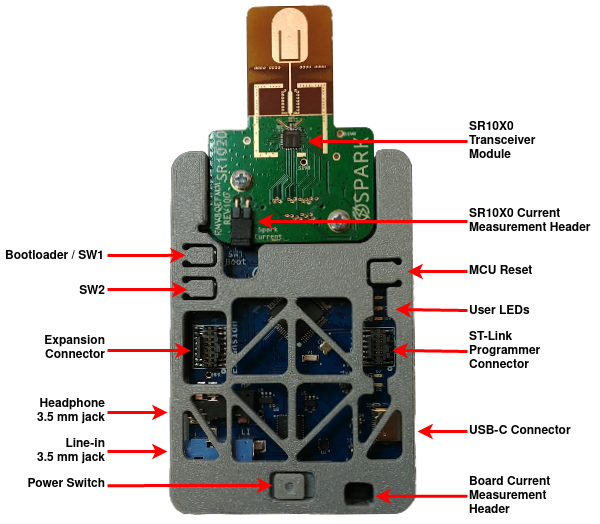
\includegraphics[width=0.7\textwidth]{images/evk picture.png}
\caption{Spark Family Evaluation Kit.}
\label{fig:spark_evk}
\end{figure}

%[Hardware Description — SPARK Microsystems SDK]
The EVK is also equipped with an audio codec and dual 3.5 mm audio jacks. While I won't discuss the EVK and radios in an audio setting, Christian Sassi evaluated the radios' latency within a haptic musical framework. The microcontroller in our EVK was the STM32G474RET6, powered by the Arm Cortex M4 32-bit RISC Core. Although it's capable of running at 170 MHz / 213 DMIPS, it offers multiple low-power modes.
% Add ref to st website
As can be noted, the EVK presents some current probes to measure electrical current. The top-left probe measures the radio's current consumption, while the bottom-right one measures the entire board's consumption - including the radio, microcontroller, codec, and interconnected PCB components.  I employed these measurement headers, paired with a power profiler, to discern their power consumption, details of which will be further discussed in the characterization chapter. Additionally, there's a JTAG expansion connector for peripherals. Via the expansion connector, it is possible to connect UART and SPI sensors. My use of the JTAG connector was limited to debugging, specifically for gauging wake-up delays by sending signals based on internal events.

\section{SDK}
\label{sec:spark_sdk}
SPARK's Software Development Kit (SDK) provides an array of development tools and sample applications. Designed to work hand-in-hand with the SPARK Evaluation Kit (EVK), the SDK equips users with clear application examples, showcasing SPARK's key libraries. It encompasses nearly all SDK features, and a board support package (BSP) further aids in testing these examples on the EVK, facilitating experimentation with SPARK's technology.
When transitioning to custom PCBs, users can adapt the provided samples, using the BSP as a reference throughout the SDK porting phase. The SDK also offers comprehensive guidelines on designing a board with their radios from the ground up. %[FOOTER NOTE TO THE SECTION OF THE WEBSITE]
The SDK encompasses three cores: Audio, Wireless, and Ranging. While Christian and I will address the Wireless Core in our characterization chapters, with a focus on different facets, only Christian delves into the Audio Core. Given the depth of the Wireless Core, I will highlight its salient aspects and features for an easier transition into the subsequent characterization chapter. For more in-depth details, refer to the SDK documentation's Wireless Core section.

% Add ref to the doc


\subsection{Transmission}

\subsubsection{Time Division Multiple Access}
The Wireless Core incorporates a network stack utilizing Time Division Multiple Access (TDMA). Adhering to the TDMA schedule is mandatory for sending packets. TDMA segments time into specific timeslots designated to certain events on every board, enhancing power efficiency. Radios can remain dormant except during their designated transmission timeslots, leveraging the more profound sleep modes available.


\subsubsection{Frequency Switching and Networks of Nodes}
Transmission channels can be altered or cycled through a predetermined list known as a channel sequence – a method known as frequency switching. This optimizes spectrum usage and ensures adherence to the FCC's regulatory emission limits. Creating a network of nodes is straightforward, with some topologies, such as the star network, being readily available. The PAN ID and node addresses facilitate this by establishing logical networks and determining packet recipients. Similar to other technologies, broadcasting packets to nodes under the same PAN is feasible.


\subsubsection{Modulation}
Two modulation types are available: Inverted On-Off Keying (IOOK) and 2-bit Pulse Modulation (2-bit PPM). While IOOK is an amplitude coding that sends a signal for a 0 bit and remains silent for a 1 bit, 2-bit PPM encodes two bits in four signals. Figure 3.3 illustrates their operation.

\begin{figure}[h]
\centering
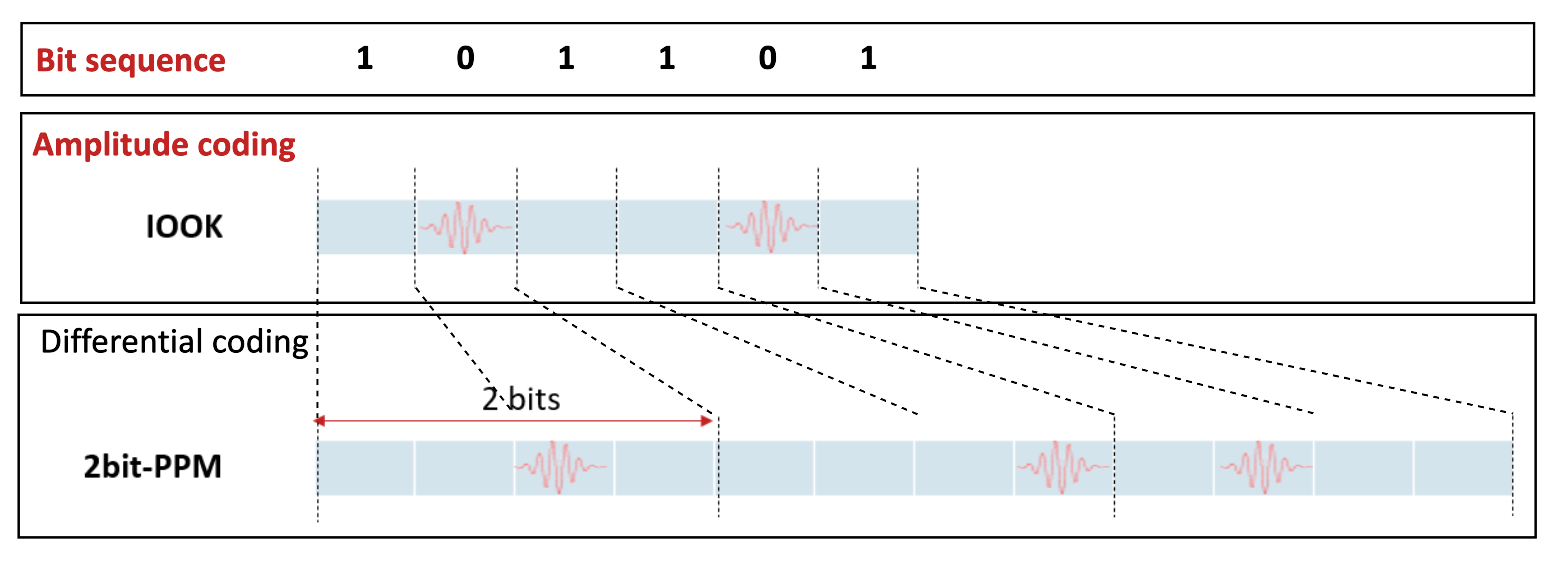
\includegraphics[width=0.7\textwidth]{images/modulation_bit_sequence.png}
\caption{Modulation Bit Sequence.}
\label{fig:modulation_bit_sequence}
\end{figure}

IOOK sends a signal when the bit is 0 and does not send anything when it is 1. Every bit is an impulse, therefore, it enables high data rates. 2bit-PPM sends four signals every two bits. As can be seen in the example in Figure 3.3, the bit sequence of six bits is divided into three blocks of four bits. Every block encodes the pair of bits.

Our characterization favored 2-bit PPM over IOOK, reserving the latter exclusively for high data rate applications.

\subsubsection{Forward Error Correction}
The system offers four distinct Forward Error Correction (FEC) levels. These non-standard levels have been detailed in the subsequent table.

\begin{table}[htbp]
\centering
\begin{tabular}{|c|c|}
\hline
FEC Level & Frame Inflation Rate \\
\hline
0 & x1 \\
\hline
1 & x1.334 \\
\hline
2 & x1.667 \\
\hline
3 & x2 \\
\hline
\end{tabular}
\caption{FEC Level versus Frame Inflation Rate} % Optional: If you want a caption for your table
\end{table}

\subsubsection{Frame Transmission}
A "Stop and Wait" mechanism exists for resending unacknowledged frames. We omitted this in our characterization to assess the packet reception rate without multiple sends.


\subsection{Sleep Modes}
The radios support three sleep modes: Idle, Shallow, and Deep. The deeper the mode, the fewer active peripherals, leading to minimized energy consumption at the cost of increased wake-up delays. A complete radio shutdown labeled the "Shutdown power state", is also available. Further insights will be shared in the characterization chapter.

\subsection{Additional Information}
The Wireless Core and its API are intricate, featuring advanced capabilities not covered here. For instance, the SDK supports fragmenting large frames, a feature employed during my distributed AEP test when the payload exceeded the 125-byte limit. Additionally, there's an "alternative channel configuration" for challenging environmental conditions and a "link throttling" feature to limit throughput and power consumption as required. While numerous other features exist, they fall outside the scope of this dissertation.

\newpage



